% ------------------------------------------------------------
% DO NOT CHANGE: BEGIN
% ------------------------------------------------------------

\documentclass [a4paper, 11pt] {article}

% ------------------------------------------------------------
% DO NOT CHANGE: BEGIN
% ------------------------------------------------------------

\usepackage[utf8]{inputenc}  
\usepackage[T1]{fontenc}  
\usepackage{lmodern}
\usepackage[english]{babel}
\usepackage{fancybox}
\usepackage{listings}
\usepackage{color}
\usepackage{graphicx,subfigure}
\usepackage[titletoc]{appendix}
\usepackage{float} % figures flottantes 
\usepackage{here} % figures flottantes
\usepackage{url}
\usepackage{enumitem}
\setlist[itemize]{noitemsep, nolistsep}
\setlist[enumerate]{noitemsep, nolistsep}
\usepackage{xcolor}
\usepackage[colorlinks=true]{hyperref}
\usepackage{tabularx}
\usepackage{minted}
\usepackage{amsmath}
\usepackage[skins,breakable]{tcolorbox}

% --------------------------------------------------------------
% Title
% --------------------------------------------------------------
\makeatletter
\newcommand\maintitle[1]{
    \quitvmode
    \hb@xt@\linewidth{
        \dimen@=1ex
        \advance\dimen@-2pt
        \leaders\hrule \@height1ex \@depth-\dimen@\hfill
        \enskip
        \textbf{#1}
        \enskip
        \leaders\hrule \@height1ex \@depth-\dimen@\hfill
    }
}
\makeatother

% --------------------------------------------------------------
% Some parameters
% --------------------------------------------------------------
\oddsidemargin =0 mm
\topmargin = -10 mm
\footskip = 20mm
\textheight = 240 mm 
\textwidth = 160mm

% --------------------------------------------------------------
% Q&A environments
% --------------------------------------------------------------

\newcommand{\emptyquestion}{Please fill this space with your question.}

\newcommand{\emptyanswer}{Please fill this space with your answer.}

\newcounter{question}

\definecolor{question_color}{RGB}{181,124,64}
\definecolor{question_color_fill}{RGB}{252,248,227}

\newcommand{\thequestionref}{No reference}

\makeatletter
\newenvironment{question}[1]
{
\refstepcounter{question}
\def\@currentlabel{{#1}}
\label{ref-question-\thequestion}
\addcontentsline{toc}{subsection}{{#1}}
\noindent
\begin{tcolorbox}[
    colframe=question_color,
    colback=question_color_fill,
    coltitle=question_color_fill,  
    title=\centering\textbf{Question #1:},
    breakable,
    width=\textwidth]
}
{   \end{tcolorbox}
}
\makeatother

\newenvironment{answer}
{
\noindent
{
\hypersetup{allcolors=question_color}
\flushleft
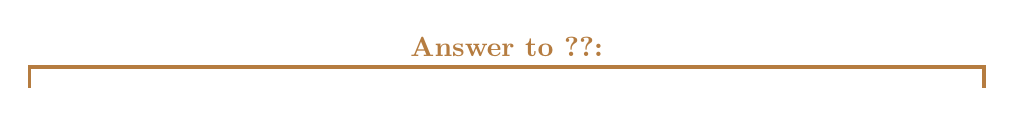
\begin{tikzpicture}
    \draw[very thick,question_color] (0,0) -- ++(0,+7.5pt)
    -- ++(\textwidth,0) node[midway,above] {\textbf{Answer to \ref{ref-question-\thequestion}:}}
    -- ++(0,-7.5pt);
\end{tikzpicture}
\vspace{-.3cm}
}
\begin{tcolorbox}[
    blanker,
    width=\textwidth,
    breakable]
}
{   \end{tcolorbox}
\vspace{-.4cm}
\flushleft

\begin{tikzpicture}
    \draw[very thick,question_color] (0,0) -- ++(0,-7.5pt)
    -- ++(\textwidth,0)
    -- ++(0,+7.5pt);
\end{tikzpicture}
}

\usepackage{tikz}

% --------------------------------------------------------------
% Code environments
% --------------------------------------------------------------
\usemintedstyle{borland}
\providecommand*{\listingautorefname}{Listing}

\newenvironment{python}
{\VerbatimEnvironment
\begin{minted}[
linenos,
% fontfamily=courier,
fontsize=\normalsize,
xleftmargin=21pt,
]{python}}
{\end{minted}}

\newcommand\py[1]{\mintinline{python}{#1}}

\newcommand\la[1]{\mintinline{latex}{#1}}

% --------------------------------------------------------------
% CELL environments
% --------------------------------------------------------------

\newcounter{cell}

\definecolor{cell_color}{RGB}{7,128,164}
\definecolor{cell_color_fill}{RGB}{247,247,247}

\newcommand{\thecellref}{No reference}

\makeatletter
\newenvironment{cell}[1]
{
\refstepcounter{cell}
\def\@currentlabel{{#1}}
\label{ref-cell-\thecell}
\addcontentsline{toc}{subsection}{\texttt{CELL N$^{\circ}${#1}}}
\noindent
\begin{tcolorbox}[
    colframe=cell_color,
    colback=cell_color_fill,
    coltitle=cell_color_fill,  
    title=\centering\texttt{CELL N$^{\circ}${#1}:},
    breakable,
    width=\textwidth]
}
{   \end{tcolorbox}
}
\makeatother

% ------------------------------------------------------------
% DO NOT CHANGE: END
% ------------------------------------------------------------
\begin{document}

    \begin{center}
        \Large
        \centering
        \maintitle{LEPL1109 - Statistics and Data Sciences}
        \textsc{\textbf{HACKATHON 2 - Diabetes health indicators}}\\
    	\vspace{0.1cm}
         Group n°XX\hfill November 29, 2024 \\
       \noindent\hrulefill
    \end{center}
    \vspace*{0.5cm}

% ------------------------------------------------------------
% DO NOT CHANGE: END
% ------------------------------------------------------------

% ------------------------------------------------------------
% FILL WITH YOUR NAMES: BEGIN
% ------------------------------------------------------------
    \hspace*{-0.75cm}
    \fbox{\parbox{\textwidth}{
    \begin{tabularx}{\textwidth}{X|X|{c}p{2cm}}
       \textbf{Lastname}  & \textbf{Firstname} & \textbf{Noma} \\
       \hline
        Decaluwé & Maxime & 50802200 \\
        Defrenne & Simon & 42242200 \\
        Mil-Homens Cavaco & Mathieu & 38282200 \\
        Peiffer & Thibaut & 47352200 \\ 
        Roekens & Raphaël & 70732200 \\ 
        Starck & Robin & 88952200 \\ 
    \end{tabularx}
    }}
% ------------------------------------------------------------
% FILL WITH YOUR NAMES: END
% ------------------------------------------------------------

% ------------------------------------------------------------
% DO NOT CHANGE: BEGIN
% ------------------------------------------------------------

    \vspace*{0.5cm}
    
    \hrule
    
    \vspace*{0.5cm}
    
    Please, read carefully the following guidelines:
    
    \begin{itemize}
        \item Answer in English, with complete sentences and correct grammar. Feel free to use grammar checker tools such as \href{https://languagetool.org/fr}{LanguageTools} free and open-source plugin;
        \item Do not modify questions, and input all answers inside \la{\begin{answer}...\end{answer}} environments;
        \item Each question should be followed by an answer;
        \item At the end of each question, there is the length of the expected answer. This is for your information but it is not too important if you do not respect these recommendations.
        \item Clearly cite every source of information (even for pictures!);
        \item Whenever possible, use the \texttt{.pdf} format when you export your images: this usually makes your report look prettier\footnote{This is because \texttt{.pdf} is a vector format, meaning that it keeps a perfect description of your image, while \texttt{.png} and other standard formats use compression. In other words, this means you can zoom as much as you want on your figure without decreasing image resolution. For simple plots, vector formats can also save a lot of memory space. On the other hand, we recommend using \texttt{.png} when you are plotting many data points: large scatter plots, heatmap, etc.};
        \item Do not forget to also submit your code on Moodle.
        \item \textbf{Reminder:} You need to belong to a group to submit your project on Moodle.
    \end{itemize}

    {
    \hypersetup{allcolors=black}
    \tableofcontents
    }   
    \clearpage

\section{Description of the project}

\subsection{Your objective}

You work in the diabetology department at \textbf{Saint Luc University Hospital}. The head of the department has asked you to find a solution for classifying and predicting \textbf{whether patients are at high risk of developing diabetes}. This will enable them to schedule an appointment with these patients to set up prevention tools. To do this, you have a database of patients who have passed through the department in recent years. In addition, the head of the department feels that the poll is too long, and would like to \textbf{reduce the number of questions while maintaining the reliability and quality of the results}. The attached \texttt{.ipynb} file will guide you in this process.\\

Your aim is to determine which characteristics are relevant and enable reliable patient classification. \textbf{Be careful}, don’t let a potential diabetic patient slip through the cracks.

\subsection{The dataset}
The dataset is a real dataset based on a questionnaire carried out in the USA some ten years ago. It contains around 70 000 entries and is a collection of 22 features individually defined in table \ref{tab:featuresList}.  

\begin{table}[htpb]
    \centering
    \hspace*{-0.5cm}
    \begin{tabular}{|c|c|c|}
    \hline
    \textbf{Features name} &\textbf{ Description }& \textbf{Range} \\\hline
    \texttt{Diabetes} & Diabetes (0:no diabetes; 1:diabetes) & \{0, 1\} \\ 
\hline
\texttt{HighBP} & High blood pressure (0:no; 1:yes) & \{0, 1\} \\ 
\hline
\texttt{HighChol} & High cholesterol (0:no; 1:yes) & \{0, 1\} \\ 
\hline
\texttt{CholCheck} & Cholesterol check in 5 years (0:no; 1:yes) & \{0, 1\} \\ 
\hline
\texttt{BMI} & Body mass index in [kg/m²] & / \\ 
\hline
\texttt{Smoker} & Smoked at least 100 cigarettes in your life~(0:no; 1:yes) & \{0, 1\} \\ 
\hline
\texttt{Stroke} & Stroke (0:no; 1:yes) & \{0, 1\} \\ 
\hline
\texttt{HeartDisease} & Heart disease (0:no; 1:yes) & \{0, 1\} \\ 
\hline
\texttt{PhysActivity} & Physical activity in past 30 days (0:no; 1:yes) & \{0, 1\} \\ 
\hline
\texttt{Fruits} & Consume fruit 1 or more times per day (0:no; 1:yes) & \{0, 1\} \\ 
\hline
\texttt{Veggies} & Consume vegetables 1 or more times per day (0:no; 1:yes) & \{0, 1\} \\ 
\hline
\texttt{Alcohol} & Heavy alcohol drinkers (0:no; 1:yes) & \{0, 1\} \\ 
\hline
\texttt{AnyHelathcare} & Health insurance (0:no; 1:yes) & \{0, 1\} \\ 
\hline
\texttt{NoDocbcCost} & No doctor because of cost (0:no; 1:yes) & \{0, 1\} \\ 
\hline
\texttt{GenHlth} & General health (1:excellent; 5:poor) & \{1, \dots, 5\} \\ 
\hline
\texttt{MenHlth} & Number of days out of the last 30 when mental health was poor & \{0, \dots, 30\} \\ 
\hline
\texttt{PhysHlth} & Number of days out of the last 30 when physical health was poor & \{0, \dots, 30\} \\ 
\hline
\texttt{DiffWalk} & Serious difficulty for walking (0:no; 1:yes) & \{0, 1\} \\ 
\hline
\texttt{Sex} & 0:female; 1:male & \{0, 1\} \\ 
\hline
\texttt{Age} & Age category (1:18-24; \dots; 13:80 or older) & \{1, \dots, 13\} \\ 
\hline
\texttt{Education} & Education level~(1:never; 6:university) & \{1, \dots, 6\} \\ 
\hline
\texttt{Income} & Income scale (1:less than \$10,000; \dots; 8:\$75,000 or more) & \{1, \dots, 8\} \\
\hline
    \end{tabular}
    \caption{Data set features}
    \label{tab:featuresList}
\end{table}
\clearpage
\section{Questions and answers (4/10)}
%------------------------------------------------------------
% DO NOT CHANGE: END
% -----------------------------------------------------------

\begin{question}{2.1}
(1/10) What happens to the precision and recall (of any method) when the threshold tends to
0? And when it tends to 1? How can you explain it?\\
\textit{Expected answer length : 8 lines.}
\end{question}
\begin{answer}\color{blue} 
% ------------------------------------------------------------
When the threshold goes to 0, recall approaches its maximum value of 1 because it is the ratio of true positives to the total actual positives, and very few (if any) false negatives occur, since almost everything is classified as positive. However, precision decreases because it is the ratio of true positives to the total predicted positives, and many false positives are included due to the broad classification of positive instances.\\

When the threshold tends to 1, precision approaches 1, as only the most confident positive predictions are retained, significantly reducing false positives. However, recall decreases because many true positives are missed, resulting in a large number of false negatives.
% ------------------------------------------------------------
\end{answer}

\begin{question}{2.2}
(1/10) Explain which precision/recall trade-off you prefer to have for the specific task asked in this hackathon: don't let a potential diabetic slip through the cracks. How should you adjust the threshold of your model to bring it closer to the desired trade-off? Should it be above or below the default threshold value of 0.5?\\
\textit{Expected answer length : 5 lines.}
\end{question}
\begin{answer}\color{blue}
% ------------------------------------------------------------
In our situation, we want to reduce as much as possible the amount of false negative, since the worst case is to predict someone is not diabetic while he is positive because that way we would ignore him while him being critically at risk. Telling someone that he is diabetic while he is not is less a problem as we could realize our mistake later on. We then want to maximize the recall of our prediction while maintaining a descent precision through f1 score. 
Knowing that the higher the threshold, the higher the precision and the lower the recall, for higher recall we need to reduce the thresold : we then need a thresold below 0.5. 
% ------------------------------------------------------------
\end{answer}

\begin{question}{2.3}
(1/10) Based on your code, select a final model that you will keep as classifier. \textbf{Justify.} \\
\textit{Expected answer length : 5 lines.}
\end{question}
\begin{answer} \color{blue}
% ------------------------------------------------------------
The model that fits our desired recall and F1-score the best, while requiring the least possible amount of questions is the linear model. Compared to the others, it reaches these values with only 5 features.
The logistic method needs as much questions as the linear for the F1-score, but it gives a lower recall. The KNN method is nearly as good as the linear for both the recall and the F1 score, but needs more features, so more questions (at least 7 questions).
\begin{center}
    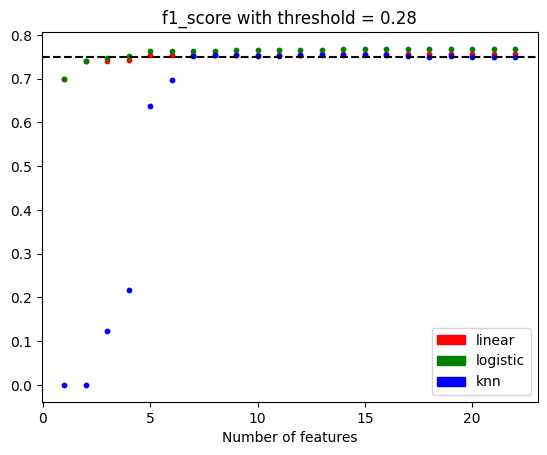
\includegraphics[width=7cm]{5_2_F.png}
    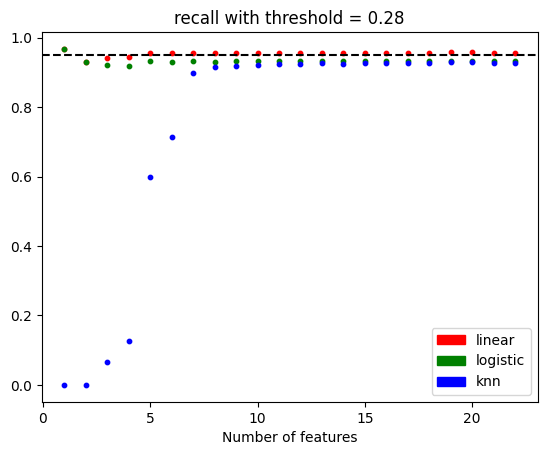
\includegraphics[width=7cm]{5_2_R.png}   
\end{center}
% ------------------------------------------------------------
\end{answer}

\begin{question}{2.4}
(1/10) Could you reduce the length of the questionnaire? If so, how many questions? Which questions? \textbf{Justify.}\\
\textit{Expected answer length : 6 lines.}
\end{question}
\begin{answer}\color{blue}
% ------------------------------------------------------------
If we use linear regression, we can reach the threshold with as few as 5 features, which means we can keep only the 5 questions 
that are the most correlated with diabetes. These questions are related to: GenHlth, HighBP, BMI, Highchol, and Age. 
Adding more features does not improve the results for either linear regression or logistic regression. For KNN, the results 
stop improving with 8 features, which means it should retain 3 additional questions related to: Diffwalk, Income, and Physhlth.
% ------------------------------------------------------------
\end{answer}


\section{Visualization (2/10)}

\begin{question}{3.1}
(2/10) To answer this question, we ask you to produce a clear, clean figure expressing a result or giving an overall vision of your work for this hackaton. Please feel free to do as you wish. Be original! The clarity, content and description of your figure will be evaluated.\\
\textit{Expected answer length : 4 lines + 1 figure.}
\end{question}
\begin{answer}\color{blue}
% ------------------------------------------------------------
% TO FILL 
% ------------------------------------------------------------
\end{answer}
\pagebreak

\end{document}

% ------------------------------------------------------------
% DO NOT CHANGE: END
% ------------------------------------------------------------